\chapter{Literature Survey}

\section{The PUF concept}
The simplest sentence to describe PUF is "A PUF is an object's fingerprint" [4]. The fingerprint can represent a specific human in the world, such as the PUF can represent
an object. The fingerprint is inherently created when people was born, and the so does PUF, which is inherently exist in an object according to unique manufacturing random variation [4].
With the representation and inherent property, the fingerprint and the PUF is said to be unclonable since it is impossible to control and predict human's fingerprint. This is an important concept for PUF. \par

This intrinsic property can be extract from chip which has PUF circuit existed inside [2]. The way PUF works is by entering a certain length of bits(so called challenge) into the PUF, and it will
generate another specific length of bits(so called response). According to the property of PUF that was discuss above, it is impossible to find two different PUF that will produce the same response when entering same challenge(See Figure 2.1).
\begin{figure}[b]
\centering
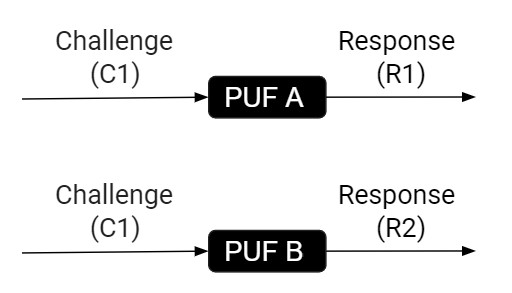
\includegraphics[width=8cm]{figures/figure1.jpg}
\caption{Different PUF that generate different response when input same challenge}
\label{fig:graph}
\end{figure}

\section{Introduce to weak and strong then authentication stage or ...}

\section{Summary}


